%\documentclass[11pt,oneside,a4paper,openright]{report}
%\usepackage[utf8]{inputenc}
%\renewcommand{\contentsname}{Indholdsfortegnelse}
%\usepackage{pdfpages}
%\usepackage{titlesec}
%\titleformat{\chapter}{\normalfont\huge}{\thechapter.}{20pt}{\huge\it}

%%%% Dokumentklassen %%%%

\documentclass[a4paper,11pt,dvipsnames,oneside,openany]{memoir} 	% Openright åbner kapitler på højresider (openany begge)
% fleqn = flush left equation - sikre at alle ligninger tvinges til venstre. I 3. semesterprojektet, skulle ligningerne stå i midten derfor er denne pakke slettet fra dokumentklassen.

\usepackage{subfiles}
\usepackage{nameref}
\usepackage{tabularx}
\usepackage{multirow}
\usepackage[table]{xcolor}


%%%% PACKAGES %%%%

%% Oversættelse og tegnsætning %%
\usepackage[utf8]{inputenc}					% Input-indkodning af tegnsæt (UTF8)
\usepackage[danish]{babel}					% Dokumentets sprog
\usepackage[T1]{fontenc}				    % Output-indkodning af tegnsæt (T1)
\usepackage{ragged2e,anyfontsize}			% Justering af elementer
%\usepackage{fixltx2e}						% Retter forskellige fejl i LaTeX-kernen
\usepackage{titletoc}
\newcommand{\nocontentsline}[3]{}
\newcommand{\tocless}[2]{\bgroup\let\addcontentsline=\nocontentsline#1{#2}\egroup}									% Giver mulighed for at fjerne section nummer i indholdsfortegnelse ved \tocless


\usepackage{lastpage}						% Total antal sider opdateres automatisk ved \pageref{LastPage}
\usepackage{tikz}							% Til at lave flow diagrammer
\usetikzlibrary{calc,trees,positioning,arrows,chains,shapes.geometric,decorations.pathreplacing,decorations.pathmorphing,shapes,matrix,shapes.symbols}				% Til at lave diagrammer
																			
%% Figurer og tabeller (floats) %%
\usepackage{graphicx} 						% Håndtering af eksterne billeder (JPG, PNG, EPS, PDF)
\usepackage{multicol}         	           	% Muliggør output i spalter
\usepackage{rotating}						% Rotation af tekst med \begin{sideways}...\end{sideways}
\usepackage{xcolor}							% Definer farver med \definecolor. Se mere: http://en.wikibooks.org/wiki/LaTeX/Colors
\usepackage{flafter}						% Sørger for at floats ikke optræder i teksten før deres reference
\let\newfloat\relax 						% Justering mellem float-pakken og memoir
\usepackage{float}							% Muliggør eksakt placering af floats, f.eks. \begin{figure}[H]
\usepackage{color, colortbl}				% Tilføjer farve til tabeller

\definecolor{Gray}{gray}{0.9}				% Definerer en farve "yeezy-gray"

%% Matematik mm. %%
\usepackage{amsmath,amssymb,stmaryrd} 		% Avancerede matematik-udvidelser
\usepackage{mathtools}						% Andre matematik- og tegnudvidelser
\usepackage{textcomp}                 		% Symbol-udvidelser (fx promille-tegn med \textperthousand)
\usepackage{rsphrase}						% Kemi-pakke til RS-saetninger, fx \rsphrase{R1}
\usepackage[version=3]{mhchem} 				% Kemi-pakke til flot og let notation af formler, f.eks. \ce{Fe2O3}
\usepackage{siunitx}						% Flot og konsistent præsentation af tal og enheder med \si{enhed} og \SI{tal}{enhed}
\sisetup{output-decimal-marker = {,}}		% Opsætning af \SI (DE for komma som decimalseparator) 

%% Referencer og kilder %%
\usepackage[danish]{varioref}				% Muliggør bl.a. krydshenvisninger med sidetal (\vref)
\usepackage{natbib}							% Udvidelse med naturvidenskabelige citationsmodeller
\usepackage{xr}							    % Referencer til eksternt dokument med \externaldocument{<NAVN>}

%% Misc. %%
\usepackage{listings}						% Placer kildekode i dokumentet med \begin{lstlisting}...\end{lstlisting}
\usepackage{lipsum}							% Dummy text \lipsum[..]
\usepackage[shortlabels]{enumitem}			% Muliggør enkelt konfiguration af lister
\usepackage{pdfpages}						% Gør det muligt at inkludere pdf-dokumenter med kommandoen \includepdf[pages={x-y}]{fil.pdf}	
\pdfoptionpdfminorversion=6					% Muliggør inkludering af pdf-dokumenter, af version 1.6 og højere
\pretolerance=2500 							% Justering af afstand mellem ord (højt tal, mindre orddeling og mere luft mellem ord)


%%%% CUSTOM SETTINGS %%%%

%% Marginer %%
\setlrmarginsandblock{3.0cm}{3.0cm}{*}		% \setlrmarginsandblock{Indbinding}{Kant}{Ratio}
\setulmarginsandblock{3.0cm}{3.0cm}{*}		% \setulmarginsandblock{Top}{Bund}{Ratio}
\checkandfixthelayout 						% Oversætter værdier til brug for andre pakker

%% Afsnitsformatering %%
\setlength{\parindent}{0mm}           		% Størrelse af indryk
\setlength{\parskip}{3mm}          			% Afstand mellem afsnit ved brug af double Enter
\linespread{1,1}							% Linjeafstand

%% Indholdsfortegnelse %%
\setsecnumdepth{subsection}		 			% Dybden af nummererede overskrifter (part/chapter/section/subsection)
\maxsecnumdepth{subsection}					% Dokumentklassens grænse for nummereringsdybde
\settocdepth{subsubsection} 					% Dybden af indholdsfortegnelsen
\setcounter{secnumdepth}{5} 				    % Ekstra subsubsection nummerering
		
%% Opsætning af listings %%
\definecolor{commentGreen}{RGB}{34,139,24}
\definecolor{stringPurple}{RGB}{208,76,239}

\lstset{language=Matlab,				    % Sprog
	basicstyle=\ttfamily\scriptsize,	    % Opsætning af teksten
	keywords={for,if,while,else,elseif,		% Nøgleord at fremhæve
			  end,break,return,case,
			  switch,function},
	keywordstyle=\color{blue},				% Opsætning af nøgleord
	commentstyle=\color{commentGreen},		% Opsætning af kommentarer
	stringstyle=\color{stringPurple},		% Opsætning af strenge
	showstringspaces=false,					% Mellemrum i strenge enten vist eller blanke
	numbers=left, numberstyle=\tiny,		    % Linjenumre
	extendedchars=true, 					    % Tillader specielle karakterer
	columns=flexible,						% Kolonnejustering
	breaklines, breakatwhitespace=true,		% Bryd lange linjer
}

%% Navngivning %%
\addto\captionsdanish{
	\renewcommand\appendixname{Appendiks}
	\renewcommand\contentsname{Indholdsfortegnelse}	
	\renewcommand\appendixpagename{Appendiks}
	\renewcommand\appendixtocname{Appendiks}
	\renewcommand\cftchaptername{\chaptername~}		% Skriver "Kapitel" foran kapitlerne i indholdsfortegnelsen
	\renewcommand\cftappendixname{\appendixname~}	% Skriver "Appendiks" foran appendiks i indholdsfortegnelsen
}

%% Kapiteludssende %%
\definecolor{numbercolor}{gray}{0.7}		            % Definerer en farve til brug til kapiteludseende
\newif\ifchapternonum

\makechapterstyle{jenor}{					        % Definerer kapiteludseende frem til ...
  \renewcommand\beforechapskip{0pt}
  \renewcommand\printchaptername{}
  \renewcommand\printchapternum{}
  \renewcommand\printchapternonum{\chapternonumtrue}
  \renewcommand\chaptitlefont{\fontfamily{pbk}\fontseries{db}\fontshape{n}\fontsize{25}{35}\selectfont\raggedleft}
  \renewcommand\chapnumfont{\fontfamily{pbk}\fontseries{m}\fontshape{n}\fontsize{1in}{0in}\selectfont\color{numbercolor}}
  \renewcommand\printchaptertitle[1]{%
    \noindent
    \ifchapternonum
    \begin{tabularx}{\textwidth}{X}
    {\let\\\newline\chaptitlefont ##1\par} 
    \end{tabularx}
    \par\vskip-2.5mm\hrule
    \else
    \begin{tabularx}{\textwidth}{Xl}
    {\parbox[b]{\linewidth}{\chaptitlefont ##1}} & \raisebox{-15pt}{\chapnumfont \thechapter}
    \end{tabularx}
    \par\vskip2mm\hrule
    \fi
  }
}											        % ... her

\chapterstyle{jenor}						        % Valg af kapiteludseende - Google 'memoir chapter styles' for alternativer

%% Sidehoved %%

\makepagestyle{AAU}							        % Definerer sidehoved og sidefod udseende frem til ...
\makepsmarks{AAU}{%
	\createmark{chapter}{left}{shownumber}{}{. \ }
	\createmark{section}{right}{shownumber}{}{. \ }
	\createplainmark{toc}{both}{\contentsname}
	\createplainmark{lof}{both}{\listfigurename}
	\createplainmark{lot}{both}{\listtablename}
	\createplainmark{bib}{both}{\bibname}
	\createplainmark{index}{both}{\indexname}
	\createplainmark{glossary}{both}{\glossaryname}
}
\nouppercaseheads									% Ingen Caps ønskes

\makeevenhead{AAU}{\small E17BAC-Synk2}{}{\leftmark}	% Definerer lige siders sidehoved (\makeevenhead{Navn}{Venstre}{Center}{Hoejre})
\makeoddhead{AAU}{\rightmark}{}{}		            % Definerer ulige siders sidehoved (\makeoddhead{Navn}{Venstre}{Center}{Højre})
\makeevenfoot{AAU}{\small \thepage \ }{}{ }						% Definerer lige siders sidefod (\makeevenfoot{Navn}{Venstre}{Center}{Højre})
\makeoddfoot{AAU}{}{}{\small \thepage \ }						% Definerer ulige siders sidefod (\makeoddfoot{Navn}{Venstre}{Center}{Højre})

\copypagestyle{AAUchap}{AAU}							% Sidehoved for kapitelsider defineres som standardsider, men med blank sidehoved
\makeoddhead{AAUchap}{}{}{}
\makeevenhead{AAUchap}{}{}{}
\makeheadrule{AAUchap}{\textwidth}{0pt}
\aliaspagestyle{chapter}{AAUchap}					% Den ny style vælges til at gælde for chapters
													% ... her
															
\pagestyle{AAU}										% Valg af sidehoved og sidefod


%%%% CUSTOM COMMANDS %%%%

%% Billede hack %%
\newcommand{\figur}[4]{
		\begin{figure}[H] \centering
			\includegraphics[width=#1\textwidth]{billeder/#2}
			\caption{#3}\label{#4}
		\end{figure} 
}

%% Specielle tegn %%
\newcommand{\decC}{^{\circ}\text{C}}
\newcommand{\dec}{^{\circ}}
\newcommand{\m}{\cdot}


%%%% ORDDELING %%%%

\hyphenation{}


%%%% Tilføjelser af min preample %%%%

% Booktabs:
% The booktabs package is needed for better looking tables. 
\usepackage{booktabs}

% Caption:
% For better looking captions. See caption documentation on how to change the format of the captions.
\usepackage[hang, font={small, it}]{caption}

% Hyperref:
% This package makes all references within your document clickable. By default, these references will become boxed and colored. This is turned back to normal with the \hypersetup command below.
\usepackage{hyperref}
	\hypersetup{colorlinks=false,pdfborder=0 0 0}

% Cleveref:
% This package automatically detects the type of reference (equation, table, etc.) when the \cref{} command is used. It then adds a word in front of the reference, i.e. Fig. in front of a reference to a figure. With the \crefname{}{}{} command, these words may be changed.
\usepackage{cleveref}
	\crefname{equation}{formel}{formler}
	\crefname{figure}{figur}{figurer}	
	\crefname{table}{tabel}{tabeller}

% Mine tilføjelser:
\usepackage{units}                        %% Bruges til at gøre fx 1/2 samlet med: \nicefrac{1}{2}.
\usepackage{tabu, longtable}              %% Bruges til tabeller.
\setlength{\tabulinesep}{1.5ex}           %% Definerer linjeafstand i tabeller.
\usepackage{enumerate}                    %% Bruges til lister.
\usepackage{tabto}                        %% Giver mulighed for TAB med fx \tabto{3em}.
\usepackage[hyphenbreaks]{breakurl}       %% Bruges til websiders url'er.
\renewcommand{\UrlFont}{                  %% Definerer url-font.
\small\ttfamily}                          %
\bibliographystyle{unsrt}                 %% Definere bibliografien. Ses til sidst i dokumentet i kapitlet Litteratur.
\usepackage{amssymb} 
\usepackage{pifont}
%\newcommand{\xmark{\ding{55}}			 % Opretter et unchecked mark

\usepackage[bottom]{footmisc}

\usetikzlibrary{%
    decorations.pathreplacing,%
    decorations.pathmorphing,%
    arrows,
    arrows.meta,
    positioning,
    shapes,
    shadows,
    shapes.geometric
    }
    \usepackage{relsize}

%\definecolor{myblue1}{RGB}{0,157,209}
\definecolor{myblue1}{rgb}{0.12, 0.56, 1.0}
\definecolor{myblue3}{RGB}{216,229,245}
%\definecolor{myblue4}{RGB}{0,149,229}
\definecolor{myblue2}{rgb}{0.19, 0.55, 0.91}
\definecolor{myblue4}{rgb}{0.08, 0.38, 0.74}
\definecolor{myred1}{rgb}{0.82, 0.1, 0.26}
\definecolor{myyellow1}{rgb}{1.0, 0.96, 0.0}
\definecolor{myyellow2}{rgb}{1.0, 0.65, 0.0}


\usepackage{pdflscape}
\usepackage{rotating}

\begin{document}
\begin{titlingpage}
\begin{center}

~ \\[3cm]

%\includegraphics[width=0.6\textwidth]{figurer/ASE}~\\[1cm]

\textsc{\LARGE Bilag 3}\\[1.5cm]

%\textsc{\Large Sundhedsteknologi}\\
%\textsc{\Large 3. semesterprojekt}\\[0.5cm]

\noindent\makebox[\linewidth]{\rule{\textwidth}{0.4pt}}\\
[0.5cm]{\Huge Kravspecifikation}
\noindent\makebox[\linewidth]{\rule{\textwidth}{0.4pt}}
\end{center}
\vfill
\begin{center}
{\large 19. december 2017}
\end{center}
\end{titlingpage}

\newpage
\tableofcontents*


\chapter{Indledning}
På baggrund af et møde med Jim Jensen fra Hammel Neurocenter, hvor udfordringer med nuværende behandling og udredning af dysfagipatienter blev diskuteret, er der udarbejdet en kravspecifikation til et system ved navnet synkerefleksmonitor(SRM). Dette system er tiltænkt til at supplere de nuværende systemer, der bruges til at udrede synke-spise problemer hos dysfagipatienter. Det skal dog for god ordens skyld understreges at systemet, der realiseres i dette projekt er på Proof-of-Concept stadie og dermed må ikke anvendes til kliniske brug. Kravet til dette system er udspecificeret af projektgruppens medlemmer uden at der er indgået en kontrakt med Hammel Neurocenter som kunde. Med andre ord er projektgruppens medlemmer ikke forpligtet til at levere et produkt til nogen. \\


Kravspecifikationen har til formål at specificere
kravene til SRM. SRM'en består af en bioimpedans måler(BI) og en EMG måler. Kravene til SRM'en er blevet prioriteret i MoSCoW analyse, hvor "must kravet" prioriteres højst. Kravspecifikationen indeholder en beskrivelse af projektets funktionelle krav, en aktør-kontekstdiagram, systemets use-cases og ikke-funktionelle krav. Til  kravspecifikationen er der lavet en accepttest, som primært har til formål at teste
de opstillede funktionelle- og ikke-funktionelle krav. Accepttesten kan ses i \textit{"bilag 9 - Accepttestspecifikation"}.


\chapter{Kravspecifikation}
%\section{Versionshistorik}
%\begin{table}[H]
%
%\begin{longtabu} to \linewidth{@{}l l l X[l]@{}}
%    Version 	&    Dato 		&    Ansvarlig 	&    Beskrivelse\\[-1ex]
%    \midrule
%    0.1 		&  	26-09-2017 	&   MBA 	&   Oprettelse og udfyldning af UC1 og Use case diagram \\
%	0.2			&	27-09-2017	&	MBA \& MHM	&	Udfyldning af UC2 - UC4 og aktør kontekstdiagram tilføjet\\
%    	0.3			&	28-09-2017	&	MBA \& MHM	&	(F)URPS+ er tilføjet\\
%    
%\label{version_Systemark}
%\end{longtabu}
% \caption {Versionshistorik}
%    \label{tab:Versionshistorik}
%\end{table}





\section{Systembeskrivelse}
Figur \ref{fig:sysbeskrivelse} viser systembeskrivelsen for SRM'en. Systemet består af et BI kredsløb og en kommerciel emg-måler, der tilsammen udgør SRM'en. Systemet fungerer ved at et sundhedspersonale foretager en BI- og EMG-måling ved at tilkoble elektroder fra hhv. BI- og EMG-måleren til et måleobjekt. Vha. en funktionsgenerator sendes en konstant strøm til måleobjektet via. BI-kredsløbet og elektroderne. Herved måles spændinger, vha. elektroderne, som opstår når forholdet mellem spænding og strøm over måleregionen. De målte spændinger omdannes til digitale værdier vha.  en A/D-konverter. Tilslut vises disse værdier på en PC-skærm i form af en graf. Sundhedspersonalet har hermed mulighed for at evaluere måleobjektets synkefrekvens. 
\subsection{Aktør kontekstdiagram}

\begin{figure}[H]
\centering
{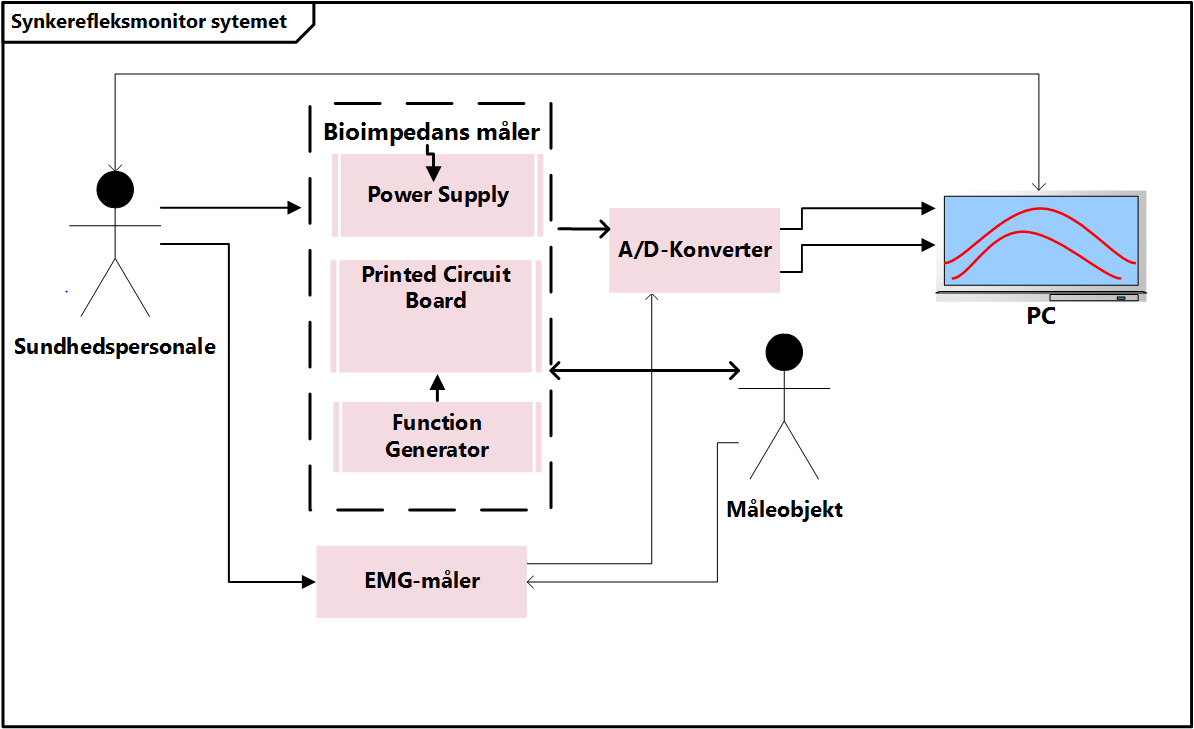
\includegraphics[width=\textwidth]
{Figure/AktoerKontextDiagram}}
\caption{Aktør-kontext diagram}
\label{fig:sysbeskrivelse}
\end{figure}  

\subsection{Aktørbeskrivelse}
\begin{table}[H]
\begin{tabularx}{\textwidth}{l l X}
     Aktørnavn	&	Type		&	Beskrivelse \\ \midrule
     Sundhedspersonale   	&  	Primær  	& 	Sundhedspersonalet tilkobler BI- og EMG-måleren til måleobjektet vha. elektroder, samt starter og afslutter målingen. Yderligere interagerer sundhedspersonalet med en brugergrænseflade.     \\ 			  \addlinespace[2mm]
     Bioimpedans-måler	&	Sekundær	& BI- måleren anvendes til at måle bioimpedans signaler fra måleobjektet  	 \\   \addlinespace[2mm]

  EMG-måler	&	Sekundær	&	EMG-måleren anvendes til at måle emg fra måleobjektet.
     \\   \addlinespace[2mm]
    
    Måleobjekt	&	Sekundær	&	Måleobjektet er kilden  hvorfra bioimpedans signalerne indhentes. Måleobjektet er tilkoblet til både BI- og EMG-måleren.
     \\   \addlinespace[2mm]
     
 A/D-konverter	&	Sekundær	&	A/D-konverterens funktion er at konvertere analog signaler fra hhv. BI-og EMG-måler  til digitale signaler.
     \\   \addlinespace[2mm]      
    PC	&	Sekundær	&	Denne brugergrænseflade bruges til at visualisere de målte signaler i graf form.
     \\   \addlinespace[2mm]
     
   
     \bottomrule                                                                                                                   
    \end{tabularx}
    \caption {Aktørbeskrivelse for hele systemet}
    \label{tab:aktoerbeskrivelse}
	
\end{table}

\pagebreak
\section{Funktionelle krav}


\subsection{Use Case diagram}

\subsubsection{Version 1.0} 


Figur \ref{UseCaseV1} viser systemets fire  usecases: Start BI-måling, Start EMG-måling, Beregn BI, Vis BI og EMG. De fire usecases udtrykker antallet af brugerscenarier som brugeren til programmet kan interagerer med på brugergrænsefladen.  Nedenstående er der detaljeret beskrivelse af de enkelte usecases gennem et fully-dressed skema. 


\begin{figure}[H]
\centering
{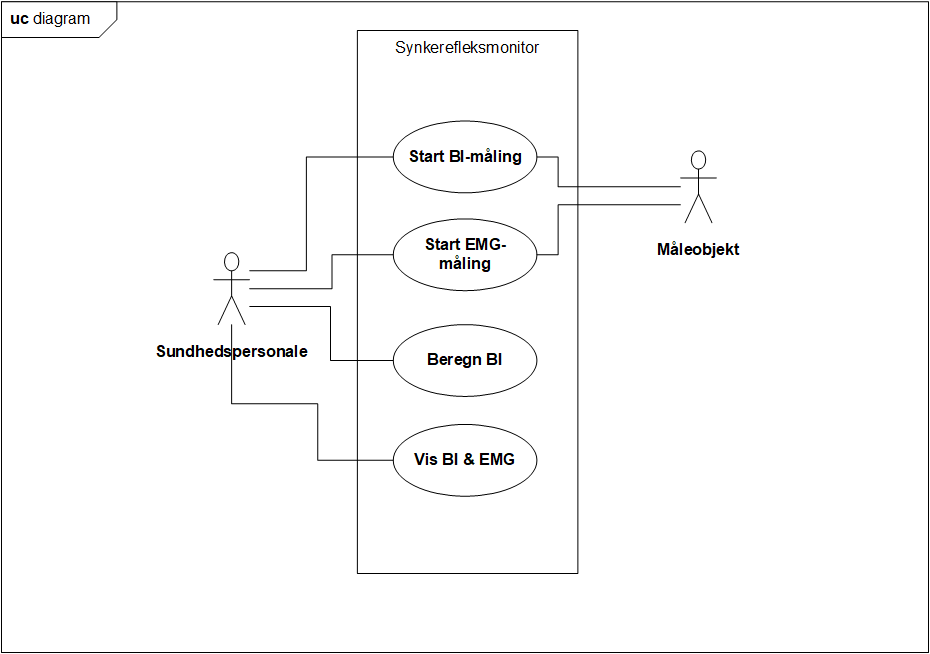
\includegraphics[width=10cm]
{Figure/usecaseDiaV1}}
\caption{UseCase diagram for synkerefleksmonitoren. Systemet består af 4 usecases, der tilsammen igangsætter, beregner og viser to målinger}
\label{UseCaseV1}
\end{figure}







Systemet består af en softwaredel, en A/D-konverter, BI-måler, EMG-måler med tilhørende hardware.






\subsection{Use Cases - fully dressed}

\subsubsection{Version 1.0}

\begin{longtabu} to \linewidth{@{}l r X[l]@{}} %UC1%
	{\large \textbf{Use Case 1}} && \\
	\toprule
	Scenarie 				&&	Hovedscenarie\\  
	Navn 					&& 	Start BI-måling\\
	Mål 					&& 	At få foretaget en BI-måling\\
	Initiering 				&& 	Startes af Sundhedspersonale\\
	Aktører 				&& 	Sundhedspersonale (primær), Måleobjekt (sekundær)\\
	Referencer 				&& 	\\
	Samtidige forekomster  	&& 	En BI-måling pr. kørsel \\
	Forudsætninger 			&&	Alle systemer er ledige og operationelle. Elektroder påsat måleobjekt og GUI-vindue er åbent\\ 
	Resultat 				&& 	BI-målingen er blevet foretaget efter ønske\\ \midrule
	Hovedscenarie 			&    1. 	&	Sundhedspersonale trykker på knappen "Start BI-måling"\\				 	
							&    2. 	& 	Systemet foretager en måling i 10 sekunder \\[-1ex]
							& 	 3.		&	 Systemet har gemt målingen i en fil \\[-1ex]
                            &&[\textit{Undtagelse 3.a:}] Systemet har ikke gemt målingen i en fil\\ \midrule
	Undtagelser 			& 3.a. & Hovedscenarie 1 i Use Case 1 gentages\\ \bottomrule
                         
	
	\caption{Fully dressed Use Case 1}
	\label{UC1}
\end{longtabu}

\begin{longtabu} to \linewidth{@{}l r X[l]@{}} %UC1%
	{\large \textbf{Use Case 2}} && \\
	\toprule
	Scenarie 				&&	Hovedscenarie\\
	Navn 					&& 	Start EMG-måling\\
	Mål 					&& 	At få foretaget en EMG-måling\\
	Initiering 				&& 	Startes af Sundhedspersonale\\
	Aktører 				&& 	Sundhedspersonale (primær), Måleobjekt (sekundær)\\
	Referencer 				&& 	\\
	Samtidige forekomster  	&& 	En EMG-måling pr. kørsel \\
	Forudsætninger 			&&	EMG-måleren er ledig og operationel. Elektroder påsat måleobjektet og GUI-vinduet er åbent\\ 
	Resultat 				&& 	EMG-målingen er blevet foretaget \\ \midrule
	Hovedscenarie 			&    1. 	&	Sundhedspersonale trykker på knappen "Start EMG-måling"\\ 				 	
							&    2. 	& 	Systemet foretager en måling i 10 sekunder \\[-1ex]
							& 	 3.		&	 Systemet har gemt målingen i en fil \\[-1ex]
                            &&[\textit{Undtagelse 3.a:}] Systemet har ikke gemt målingen i en fil\\ \midrule
	Undtagelser 			& 3.a. & Hovedscenarie 1 i Use Case 2 gentages\\ \bottomrule
	\caption{Fully dressed Use Case 2}
	\label{UC2}
\end{longtabu}

\begin{longtabu} to \linewidth{@{}l r X[l]@{}} %UC1%
	{\large \textbf{Use Case 3}} && \\
	\toprule
	Scenarie 				&&	Hovedscenarie\\
	Navn 					&& 	Beregn BI\\
	Mål 					&& 	At få beregnet BI\\
	Initiering 				&& 	Startes af Sundhedspersonale\\
	Aktører 				&& 	Sundhedspersonale (primær)\\
	Referencer 				&& 	Use Case 1\\
	Samtidige forekomster  	&& 	En BI-beregning pr. kørsel \\
	Forudsætninger 			&&	Use case 1 er foretaget\\ 
	Resultat 				&& 	BI-beregningen er foretaget \\ \midrule
	Hovedscenarie 			&    1. 	&	Sundhedspersonale trykker på knappen "Beregn-BI"\\	
							&    2. 	& 	Systemet har gemt BI-beregningen i en fil\\
                             &&[\textit{Undtagelse 2.a:}] Systemet har ikke gemt BI-beregningen i en fil\\ \midrule
Undtagelser 			& 2.a. & Hovedscenarie 1 i Use Case 3 gentages\\  \\ \bottomrule
	
	\caption{Fully dressed Use Case 3}
	\label{UC3}
\end{longtabu}

\begin{longtabu} to \linewidth{@{}l r X[l]@{}} %UC1%
	{\large \textbf{Use Case 4}} && \\
	\toprule
	Scenarie 				&&	Hovedscenarie\\
	Navn 					&& 	Vis BI \& EMG\\
	Mål 					&& 	At få vist BI- \& EMG-måling over tid på en graf\\
	Initiering 				&& 	Startes af Sundhedspersonale\\
	Aktører 				&& 	Sundhedspersonale (primær)\\
	Referencer 				&& 	\\
	Samtidige forekomster  	&& 	En graf pr. kørsel \\
	Forudsætninger 			&&	Use case 2 og 3 er foretaget\\ 
	Resultat 				&& 	Grafen er vist efter ønske\\ \midrule
	Hovedscenarie 			&    1. 	&	Sundhedspersonale trykker på knappen "Vis BI \& EMG"\\				 	
							&    2. 	& 	Grafen vises i GUI-vinduet\\
	Undtagelser 			&			& 	-  \\ \bottomrule
	
	\caption{Fully dressed Use Case 4}
	\label{UC4}
\end{longtabu}

\subsection{Use Case diagram }
\subsubsection{Version 1.1} 
\begin{figure}[H]
\centering
{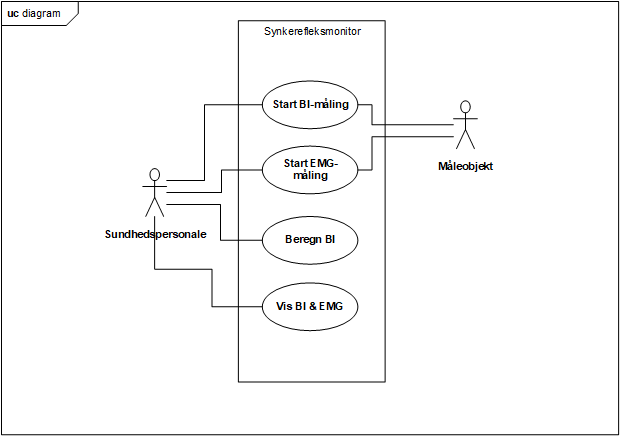
\includegraphics[width=10cm]
{Figure/usecasediagram}}
\caption{UseCase diagram for synkerefleksmonitoren. Systemet består af to usecases, der starter og gemmer målinger}
\label{Use Case diagram}
\end{figure}


\subsection{Use Cases - fully dressed}

\subsubsection{Version 1.1} 






\section{Ikke-funktionelle krav}






nielsen \cite{NielsenUsabilityUsability}

\subsection{(F)URPS+}

\textbf{Usability}
\begin{enumerate}
\item Sundhedspersonalet skal kunne anvende synkerefleksmonitoren efter 10 minutters instruktion. 
\item Sundhedspersonalet skal kunne efter endt introduktion til synkerefleksmonitoren foretage en måling uden fejl.
\item Sundhedspersonalet skal kunne efter en periode, på en uge væk fra synkerefleksmonitoren, foretage en måling uden fejl.
\item Sundhedspersonalet får mulighed for, at give karakter til GUI-designet på en skala fra 1-5, hvor 5 er yderst tilfredsstillende.
\item Sundhedspersonalet skal kunne aflæse graferne fra GUI'en på 2 meters afstand. 
\end{enumerate}
                                                                                                
\textbf{Reliability}
\begin{enumerate}[resume]
\item Det skal maksimalt tage 5 timer at gendanne Synkerefleksmonitor (MTTR - Mean Time To Restore).
\item Synkerefleksmonitor skal have en oppetid uden nedbrud på minimum 1 dag (24 timer) (MTBF - Mean Time Between Failure).  
\item Synkerefleksmonitor skal have en oppetid/køretid på: 
\end{enumerate}


\begin{equation}
Availability = \frac{MTBF}{MTBF+MTTR}\cdot100 = \frac{24}{24+5}\cdot100 = 82,76 \%
\end{equation}

					
\textbf{Performance}
\begin{enumerate}[resume]
\item Synkerefleksmonitorens hardware skal kunne tændes indenfor 3 minutter.
\item Synkerefleksmonitorens GUI skal kunne vises indenfor 3 minutter.
\item GUI'ens responstid skal maksimum være 10 sekunder.

\end{enumerate}


\textbf{Supportability}
\begin{enumerate}[resume]
\item Sundhedspersonalet skal kunne udskifte batterierne til hardwaren inden for 2 minutter.
\item Sundhedspersonalet skal kunne udskifte elektroderne inden for 2 minutter.
\item Softwaren skal opbygges med lav samhørlighed.
\end{enumerate}

\newpage
\bibliography{library}
\newpage
\listoffigures
\newpage
\listoftables

\end{document}